\newpage

\section{Backend and API Integration}
\label{sec:backend_api}

The backend infrastructure is a critical component of our AI-powered mobile application, enabling secure data handling, user management, and seamless communication between the mobile client and AI services. Built around Appwrite—a self-hosted backend-as-a-service (BaaS) platform—the system benefits from a robust, modular, and scalable architecture.

\subsection{Appwrite as Backend-as-a-Service (BaaS)}

Appwrite serves as the core backend platform, providing essential services such as authentication, database storage, file handling, serverless computing, and real-time updates. It supports structured data for user profiles and health records, encrypted storage for audio and medical files, and custom functions for executing AI-based health analysis.

The architecture shown in Figure~\ref{fig:appwrite_backend} depicts how the Flutter-based mobile frontend communicates with Appwrite services over secure HTTPS, enabling a seamless flow of authentication, data storage, and diagnostic processing. Each backend service operates independently while being orchestrated via the Appwrite API Gateway, which manages routing and authentication for all client requests.

\begin{figure}[H]
    \centering
    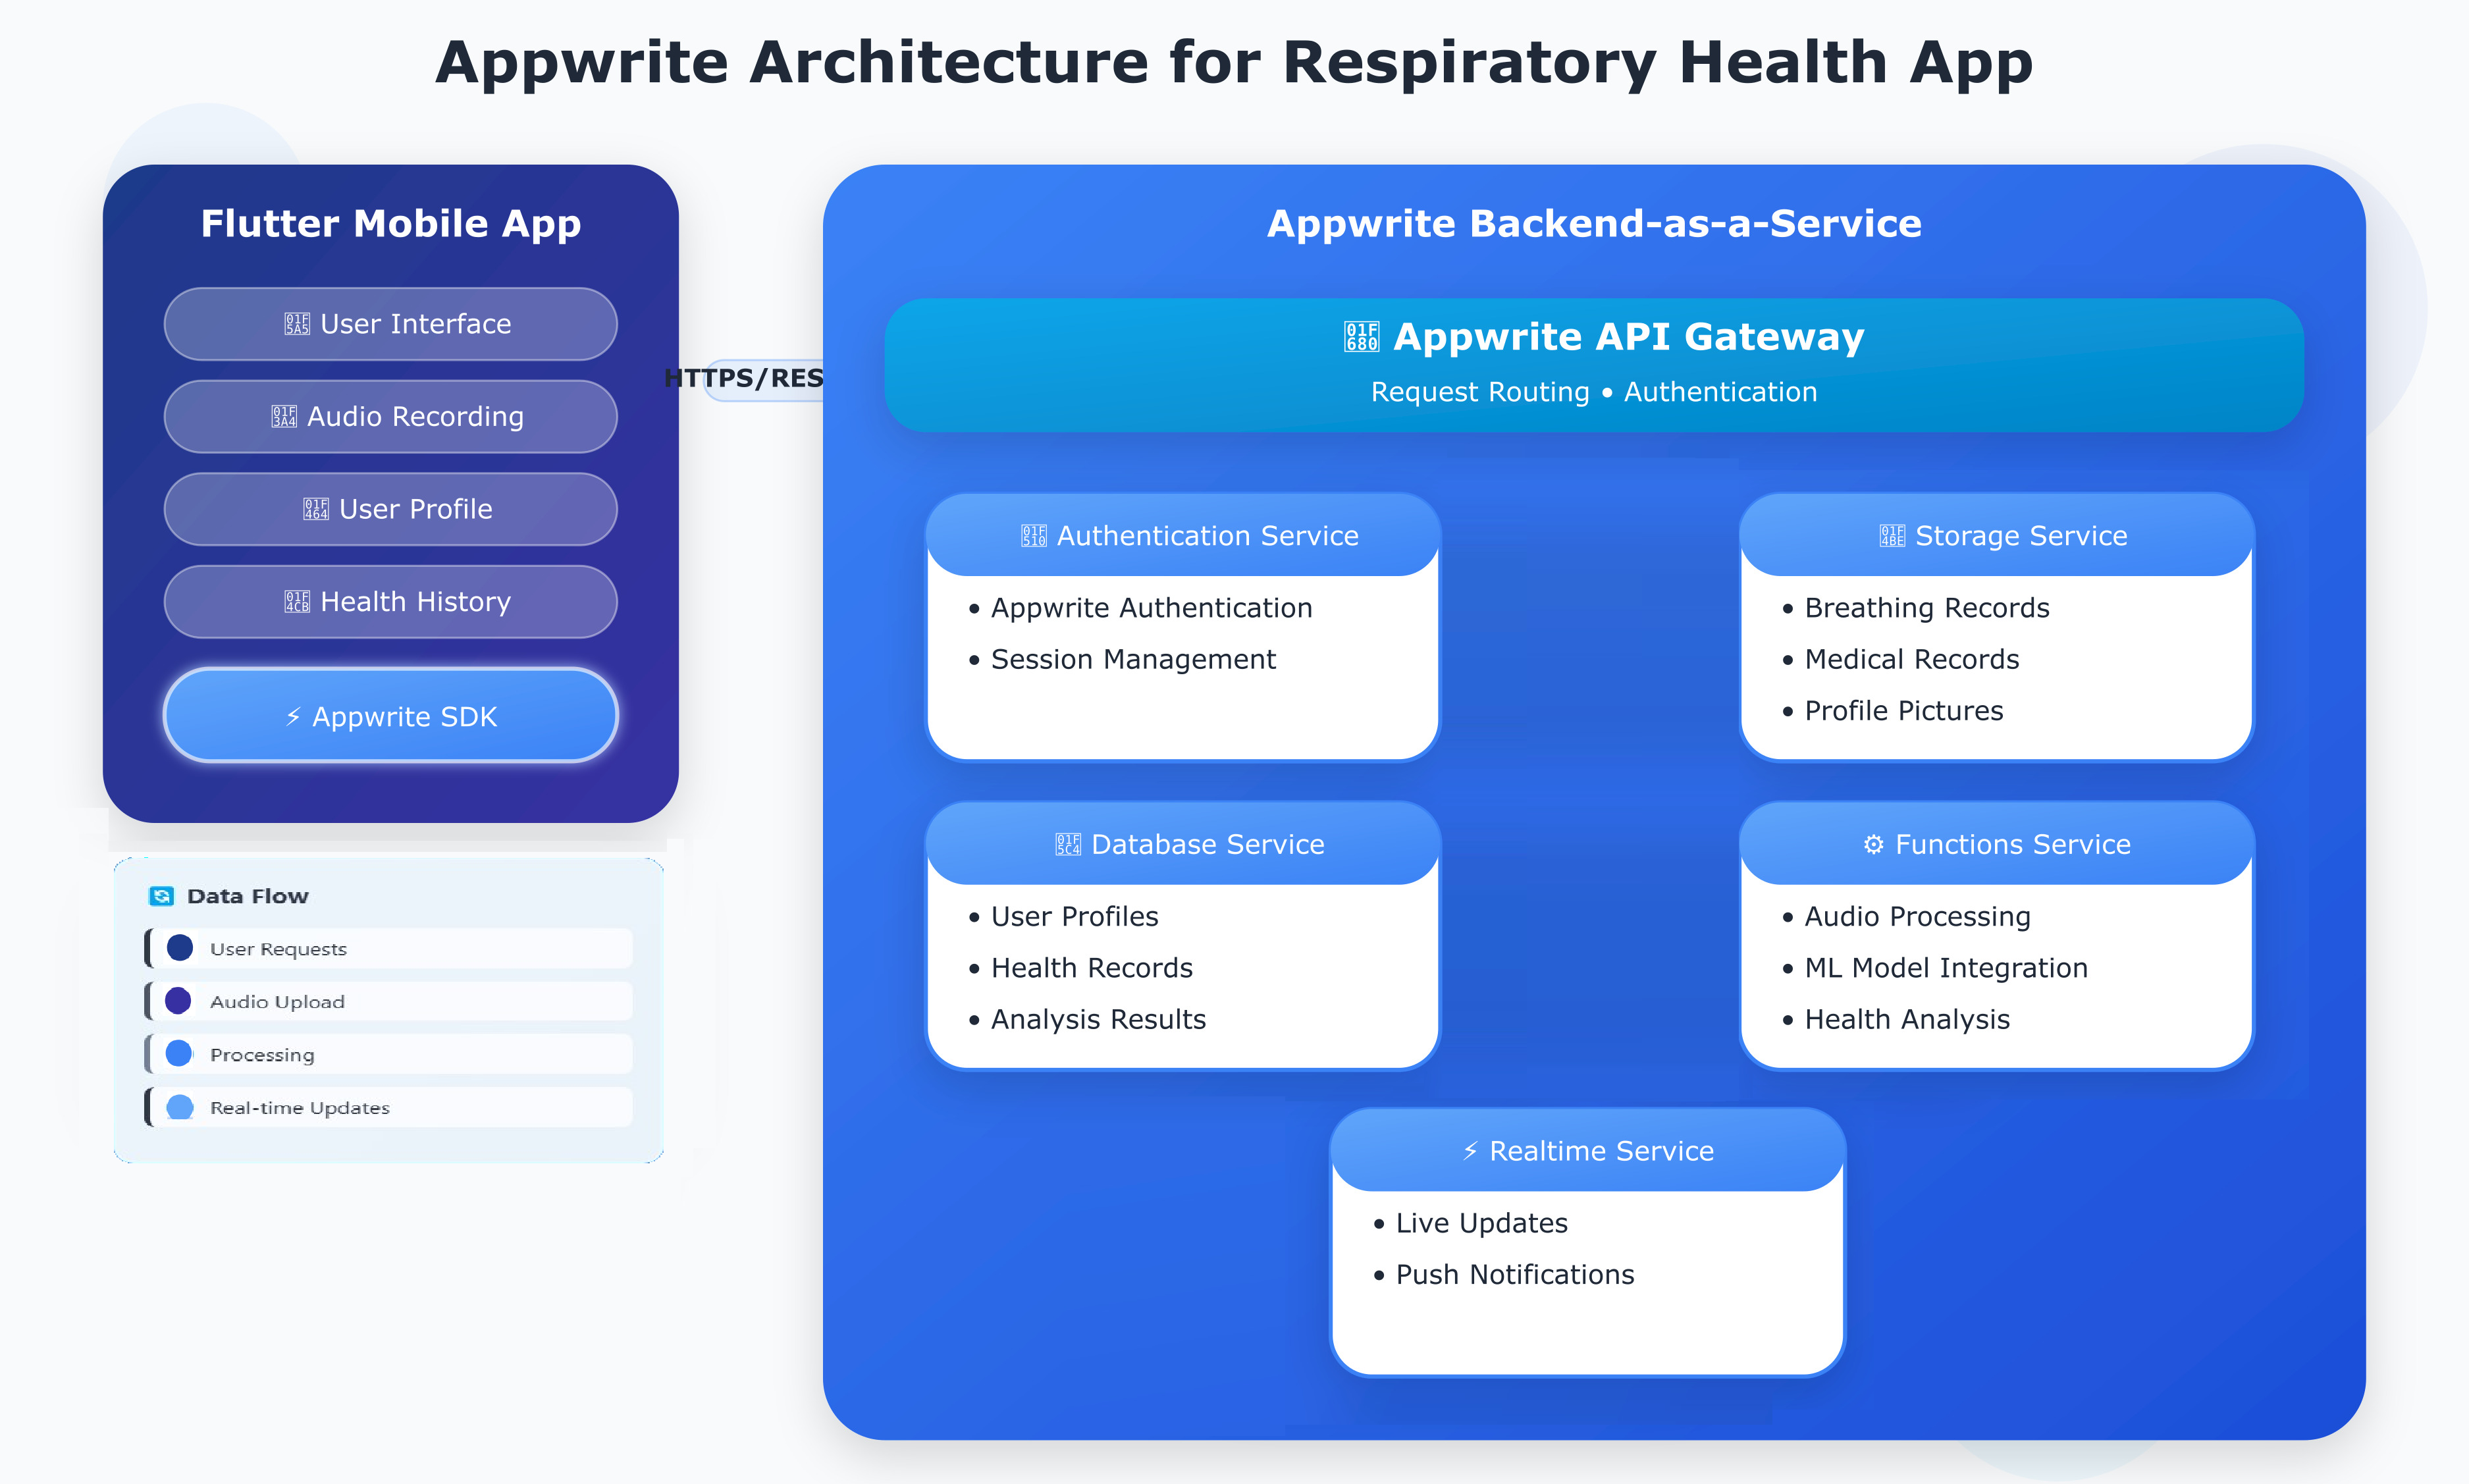
\includegraphics[width=0.95\textwidth]{images/backend/apprwite_architecture.png}
    \caption{Appwrite-Based Backend Architecture}
    \label{fig:appwrite_backend}
\end{figure}

\subsection{Authentication and Session Management}

User authentication is handled through Appwrite’s secure email-password mechanism. Upon successful login or registration, the client receives a session token, which is used to authorize all subsequent requests. This approach ensures privacy, data isolation, and secure access to personalized health information.

\subsection{Diagnosis Submission and File Handling}

When a user initiates a new diagnosis, the application uploads the audio recording and any supplementary files to Appwrite’s storage service. These assets are then linked to a new diagnosis document in the Appwrite database, which contains relevant metadata such as the timestamp, reported symptoms, and user ID.

\subsection{Triggering AI Inference}

Following submission, an Appwrite function is triggered asynchronously. This serverless function retrieves the uploaded audio file, forwards it to the AI inference engine through a secure REST API, and receives a structured JSON response. The results—comprising predicted conditions, confidence scores, and supplementary data—are saved back to the corresponding document in the database.

\subsection{Result Synchronization with the Mobile App}

To ensure responsiveness, the mobile app routinely polls the backend for updates to diagnosis records. When inference results are available, the interface updates to reflect the final diagnosis. Optionally, Appwrite’s real-time services can push changes to the client directly, allowing live updates and improved interactivity in future versions.

\subsection{Summary}

The backend architecture effectively bridges the user-facing application with the AI-driven analysis pipeline. Appwrite provides a secure, modular environment for managing identity, health data, and inference workflows. This integration enables scalable diagnostics while maintaining user privacy and system extensibility.
